\PassOptionsToPackage{unicode=true}{hyperref} % options for packages loaded elsewhere
\PassOptionsToPackage{hyphens}{url}
%
\documentclass[onecolumn]{article}
\usepackage{lmodern}
\usepackage{amssymb,amsmath}
\usepackage{ifxetex,ifluatex}
\usepackage{fixltx2e} % provides \textsubscript
\ifnum 0\ifxetex 1\fi\ifluatex 1\fi=0 % if pdftex
  \usepackage[T1]{fontenc}
  \usepackage[utf8]{inputenc}
  \usepackage{textcomp} % provides euro and other symbols
\else % if luatex or xelatex
  \usepackage{unicode-math}
  \defaultfontfeatures{Ligatures=TeX,Scale=MatchLowercase}
\fi
% use upquote if available, for straight quotes in verbatim environments
\IfFileExists{upquote.sty}{\usepackage{upquote}}{}
% use microtype if available
\IfFileExists{microtype.sty}{%
\usepackage[]{microtype}
\UseMicrotypeSet[protrusion]{basicmath} % disable protrusion for tt fonts
}{}
\IfFileExists{parskip.sty}{%
\usepackage{parskip}
}{% else
\setlength{\parindent}{0pt}
\setlength{\parskip}{6pt plus 2pt minus 1pt}
}
\usepackage{hyperref}
\hypersetup{
            pdftitle={Supplementary figures and code},
            pdfauthor={Greg Gloor},
            pdfborder={0 0 0},
            breaklinks=true}
\urlstyle{same}  % don't use monospace font for urls
\usepackage[margin=2cm]{geometry}
\usepackage{longtable,booktabs}
% Fix footnotes in tables (requires footnote package)
\IfFileExists{footnote.sty}{\usepackage{footnote}\makesavenoteenv{longtable}}{}
\usepackage{graphicx,grffile}
\makeatletter
\def\maxwidth{\ifdim\Gin@nat@width>\linewidth\linewidth\else\Gin@nat@width\fi}
\def\maxheight{\ifdim\Gin@nat@height>\textheight\textheight\else\Gin@nat@height\fi}
\makeatother
% Scale images if necessary, so that they will not overflow the page
% margins by default, and it is still possible to overwrite the defaults
% using explicit options in \includegraphics[width, height, ...]{}
\setkeys{Gin}{width=\maxwidth,height=\maxheight,keepaspectratio}
\setlength{\emergencystretch}{3em}  % prevent overfull lines
\providecommand{\tightlist}{%
  \setlength{\itemsep}{0pt}\setlength{\parskip}{0pt}}
\setcounter{secnumdepth}{0}
% Redefines (sub)paragraphs to behave more like sections
\ifx\paragraph\undefined\else
\let\oldparagraph\paragraph
\renewcommand{\paragraph}[1]{\oldparagraph{#1}\mbox{}}
\fi
\ifx\subparagraph\undefined\else
\let\oldsubparagraph\subparagraph
\renewcommand{\subparagraph}[1]{\oldsubparagraph{#1}\mbox{}}
\fi

% set default figure placement to htbp
\makeatletter
\def\fps@figure{htbp}
\makeatother

\usepackage{geometry}
\usepackage{amsmath}
\usepackage{color}
\newcommand{\ith}[1]{ #1\textsuperscript{th}\ }
\newcommand{\vect}[1]{\vec{\textbf{#1}}}
\setlength{\columnsep}{18pt} 

\setlength\textwidth{5.5in}
 \setlength\marginparwidth{1.5in}

\title{Supplementary figures and code}
\author{Greg Gloor}
\date{04 March, 2021}

\begin{document}
\maketitle

{
\setcounter{tocdepth}{2}
\tableofcontents
}
\hypertarget{about-this-document}{%
\section{About this document}\label{about-this-document}}

This document is an .Rmd document and can be found at:

github.com/ggloor/effect/effect\_supplement.Rmd

The document is requires Rmarkdown and an installation of \LaTeX to work
properly. It contains interspersed markdown and R code that may be
compiled into a pdf document and supports the figures and assertions in
the main article. R code is not exposed in the pdf document but is
either referred to by \texttt{R-code.r}, or by \texttt{R-block-n}. Both
are are annotated R code chunks. The former are in the supplementary
\texttt{code} directory, and the latter are interspersed in the
document. Both are provided so that the interested reader can work
through as need or interest arises.

\hypertarget{r-packages-required}{%
\subsection{R packages required}\label{r-packages-required}}

We will need the following R packages and add-ons (\texttt{R-block-1}).
The code chunk \texttt{code/setup.r} processes the input and output
files for analysis, and contains pointers to the files used to create
the analysis data that follows.

\begin{enumerate}
\def\labelenumi{\arabic{enumi}.}
\tightlist
\item
  knitr (CRAN)
\item
  Rmarkdown (CRAN)
\item
  ALDEx2 (Bioconductor)
\item
  CoDaSeq (github.com/ggloor/CoDaSeq)
\item
  source(`code/setup.r')
\end{enumerate}

\begin{verbatim}
## Warning in polygon(d.2, col = rgb(1, 0, 0, 0.2), border = "red"): semi-
## transparency is not supported on this device: reported only once per page
\end{verbatim}

\hypertarget{datasets}{%
\subsection{Datasets}\label{datasets}}

The transcriptome dataset in \texttt{data/barton\_agg.tsv} is a
48-replicate, two-condition RNA-seq that was done to compare the
transcriptome of the BY4741 strain (wild-type) of
\emph{Saccharomyces cerevisiae} to that of a SNF2 knockout mutant strain
from the same genetic background (Gierliński \emph{et al.}, 2015). The
96 samples were prepared in four batches of 24 samples. RNA was
extracted from each of the biological replicates and enriched for
polyadenylated RNA. ERCC external RNA spike-in mix was added to each
sample (Jiang \emph{et al.}, 2011). The RNA in each sample was
fragmented and reverse transcribed to cDNA. The cDNA corresponding to
each biological replicate was sequenced on seven lanes of an Illumina
HiSeq 2000, thus giving seven technical replicates for each biological
replicate. The sequencing data was downloaded from the European
Nucleotide Archive under the project ID PRJEB5348. Each of the 672 fastq
files, corresponding to one of the technical replicates was aligned to
the complete and annotated yeast genome (NCBI project accession:
PRJNA128), that had been modified to include the sequences for the 96
ERCC external RNA spike-ins (NIST SRM number: 2374), using bowtie2
v2.1.0 (Langmead and Salzberg, 2012){]} with the default options. For
each of the 672 replicates, the counts of sequencing reads mapped to
each gene and to each of the ERCC external RNA spike-in sequences was
determined using HTSeq v0.6.1 (Anders \emph{et al.}, 2015). All reads
with an alignment quality less than 0 were omitted. For each biological
replicate, the counts for its technical replicates were aggregated by
summing. Since the experiment done by (Gierliński \emph{et al.}, 2015)
enriched for polyadenylated RNA, counts for sequences that had been
mapped to genes annotated as rRNA were removed as they were assumed to
only contribute noise to the data.

The 16S rRNA gene sequencing dataset were obtained from the
supplementary material of (Bian \emph{et al.}) located at:
\url{https://doi.org/10.6084/m9.figshare.4535660}. The two groups were
extracted from the entire dataset using the extraction code in
\texttt{data/effect\_reproducibility\_16S.R}. Samples were filtered to
remove OTUs that were not observed in any sample and the count table
saved in \texttt{data/tiyaini\_pup\_vs\_ys.Rdata} for use.

For each dataset, a reference set of significant features for ALDEx2 was
generated by performing and collecting 100 replicates of the entire
dataset comparison using the code in
\texttt{code\textbackslash{}effect\_reproducibility.R} and
\texttt{code\textbackslash{}effect\_reproducibility\_16S.R}, a parallel
analysis of the transcriptome dataset with \texttt{edgeR} (Anders
\emph{et al.}, 2013) was conducted using
\texttt{code\textbackslash{}effect\_reproducibility\_edgeR.r}. Once the
reference set was collected, we conducted 100 replicates of balanced
sample size comparisons for each sample size between 2 and 40 samples
for the transcriptome data and between 2 and 100 samples for the 16S
rRNA gene sequencing data. We collected all features that were
identified as passing the significance cutoffs chosen and saved them for
use.

\hypertarget{reproducing-the-analysis}{%
\subsection{Reproducing the analysis}\label{reproducing-the-analysis}}

From an R command prompt you can compile this document into PDF if you
have \LaTeX and pandoc installed:

\texttt{rmarkdown::render(\textquotesingle{}effect\_supplement.Rmd\textquotesingle{})},
or you can do the same in bash (R -e
``rmarkdown::render(`effect\_supplement.Rmd')'') or you can open the
file in RStudio and compile in that environment.

\clearpage

\hypertarget{effect-size}{%
\section{Effect size}\label{effect-size}}

Cohen's d, and similar statistics of a standardized mean difference
(here-after effect size), use summary statistics to estimate the effect
size (Hedges and Olkin, 1985; Cohen, 2013). The standard equation is in
equation 1 and broadly speaking an effect size of this type is the ratio
of the difference \(\delta\) and the dispersion \(\sigma\) of two
datasets.

\begin{equation}
    z = \frac{\mu_a - \mu_b}{\sigma} = \frac{\delta}{\sigma}
    \label{effect}
\end{equation}

In equation 1 all values are summary statistics from distributions \(a\)
and \(b\), and the utility of \(z\) thus depends upon how well the
assumptions of each summary statistic fits the underlying distributions.
If \(z\) is calculated from the mean and standard deviation of a Normal
distribution, then \(z\) is the number of \(z\) scores that separate the
two mean values.

\hypertarget{effect-size-vs-difference}{%
\subsection{Effect size vs Difference}\label{effect-size-vs-difference}}

\begin{figure}
\centering
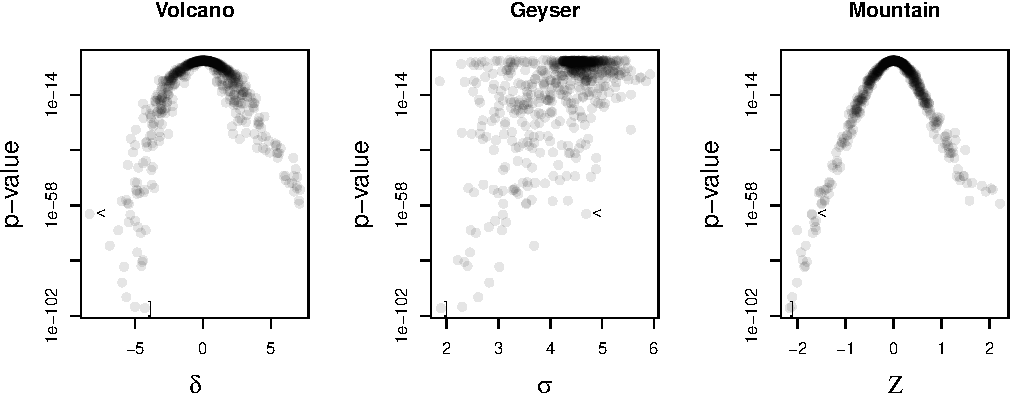
\includegraphics{effect_supplement_files/figure-latex/volcvseff-1.pdf}
\caption{The relationship between a p-value and the elements that are
used to calculate the p-value, \(\delta\) and \(\sigma\) are shown in
the left two panels labelled Volcano and Geyser. The relationship
between a p-value and \(z\) is in the third panel, labelled Mountain.
The arrow locates the feature with the largest magnitude of change, and
the square bracket locates the feature with the largest effect size and
lowest p-value.}
\end{figure}

It is worth pointing out that a p-value is not a measure of magnitude of
change (or difference), nor is a p-value a standard measure of effect
size. Nevertheless, both p-values and difference are widely used in the
high throughput sequencing literature as proxies for effect size. The
most obvious example of this is when investigators use a Volcano plot
which shows the relationship between p-values and the difference between
groups (Cui and Churchill, 2003).

Recall that one common way a p-value is calculated is from the
t-statistic which has the general form shown in equation 2. Comparing
equation 1 and equation 2 we see that the denominator is different;
\(\sigma\) is the denominator when calculating \(z\), and the square
root of \(\sigma\) divided by the sample size \(\mathrm{N}\) is the
denominator when calculating \(t\). Thus, p-values are not stable
estimates of effect size, but rather are strongly dependent on sample
size.

\begin{equation}
    t = \frac{\mu_a - \mu_b}{\sqrt{\sigma / \mathrm{N}}} = \frac{\delta}{\sqrt{\sigma / \mathrm{N}}}
    \label{ttest}
\end{equation}

The Volcano plot in Figure 1 shows the relationship between p-values and
\(\sigma\) or \(\delta\), and between p-values and \(z\). We see that
the relationship between p-values and \(\delta\) (difference) appears to
be relatively strong in the Volcano plot. However, note that there is
considerable scatter around the relationship, such that the feature with
the largest difference (denoted by the `\textless{}'), does not have the
lowest p-value. This is troubling, and the reason for this becomes
evident when we examine the `Geyser' plot which shows that this feature
has a very large dispersion. Finally, we can see in the `Mountain' plot
that the feature has a large, but not the largest standardized mean
difference. Conversely, the feature with the lowest p-value (denoted by
the `{]}') does not have the largest \(\delta\), but has a combination
of a large \(\delta\) and a small \(\sigma\). This is the information we
actually want to determine, and we can see that this feature has the
largest absolute effect size.

\hypertarget{the-distribution-effect-size-mathcalz}{%
\subsection{\texorpdfstring{The distribution effect size
(\(\mathcal{Z}\))}{The distribution effect size (\textbackslash{}mathcal\{Z\})}}\label{the-distribution-effect-size-mathcalz}}

We now introduce and demonstrate the properties of the \(\mathcal{Z}\).
The metric was first developed and used as a convenience for meta-RNAseq
(Fernandes \emph{et al.}, 2013; Macklaim \emph{et al.}, 2013) and later
for microbiome analyses (eg. Fernandes \emph{et al.}, 2014; Bian
\emph{et al.}), however, these publications did not investigate its
properties. The purpose of \(\mathcal{Z}\) is to determine the
standardized difference between two distributions, rather than the
standardized difference between the means (or midpoints) of the
distributions. Let us briefly explain the difference.

The approach taken by \(\mathcal{Z}\) is to calculate the median of the
standardized difference of the distributions, \(\vec{\varepsilon}\). We
will use vector format and start with our two distributions represented
as \(\vec{a}\) and \(\vec{b}\). The \(\mathcal{Z}\) metric is calculated
as in equation \ref{Fe} from the outputs of the prior equations 3 and 4.
Note that both the difference and dispersion estimates are vectors and
not point estimates.

\begin{align}
    \vec{\delta} = \vec{a} - \vec{b}\\
    \vec{\sigma} =  max \{ \lvert \vec{a} - \boldsymbol{\rho} \vec{a}  \rvert ,\lvert \vec{b} -\boldsymbol{\rho} \vec{b} \rvert \}\\
  \vec{\varepsilon} =  \frac{ \vec{\delta} }{ \vec{\sigma} }\\
  \mathcal{Z} = \mathrm{med} (\vec{\varepsilon})
  \label{Fe}
\end{align}

In equations 3-5, we use \(\mathrm{max}\) to refer to the maximum value
at each position in the vector, \(\mathrm{med}\) to refer to the median
of the vector, \(\lvert~\rvert\) to indicated the absolute value of the
elements in the enclosed vector, and \(\boldsymbol{\rho}\) to denote one
or more random permutations of the associated vector.

Note that both the numerator and the denominator in equation 5 are
vectors as is the result since we are calculating the ratio of the
vector values element-wise. The numerator, \(\vec{\delta}\), is simply
the signed difference between the distributions in \(\vec{a}\) and
\(\vec{b}\), and the denominator, \(\vec{\sigma}\), is the maximum
absolute difference, a novel estimate of the pooled dispersion of the
distributions. The \(\vec{\sigma}\) metric is necessary since there is
no vector-wise dispersion estimate in common use.

\hypertarget{properties-of-the-median-of-vecdelta-msd}{%
\subsection{\texorpdfstring{Properties of the median of
\(\vec{\delta}\),
MSD}{Properties of the median of \textbackslash{}vec\{\textbackslash{}delta\}, MSD}}\label{properties-of-the-median-of-vecdelta-msd}}

The midpoints of both \(\vec{\delta}\) and \(\vec{\sigma}\) have
meaning, and are calculated by ALDEx2. The median of \(\vec{\delta}\) is
the median signed difference (MSD, \texttt{diff.btw} in ALDEX2) and the
median of \(\vec{\sigma}\), or the median of the maximum absolute
difference (MMAD), is the dispersion statistic \texttt{diff.win}
returned by ALDEx2. The code contained in \texttt{R-block-2}, and Figure
2 shows the behaviour of the MSD relative to the difference of means for
three distributions as a measure of location. We can see that the two
methods are essentially equivalent except in the case of a Cauchy
distribution, where the difference in means clearly fails to provide an
reliable estimate of location. Thus, the median of \(\vec{\delta}\) is
an efficient and safe choice to determine location regardless of the
underlying distribution.

\begin{figure}
\centering
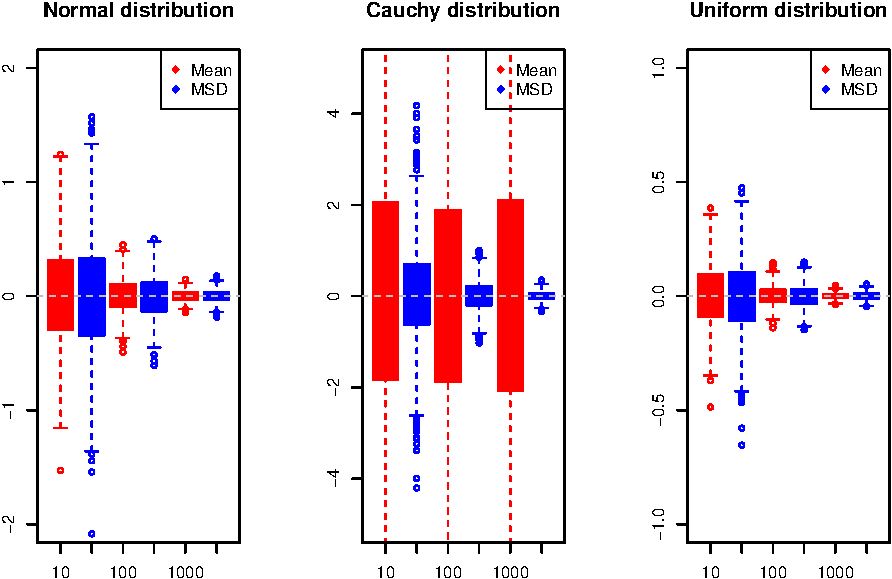
\includegraphics{effect_supplement_files/figure-latex/R-block-2-1.pdf}
\caption{Boxplots of residual values of the difference in means, or the
median of \(\vec{\delta}\) (MSD) for 1000 trials between two random
distributions with a known difference of 1. The number of samples in the
distributions was 10, 100 or 1000. A perfect estimator of location would
have a residual of 0 without any variation. The difference in means
(Mean, red) and the median of the difference vector (MSD) return very
similar results except in the case of a Cauchy distribution, where the
MSD is clearly preferable. The y-axis of the Cauchy distribution plot
has been truncated since the limit of the difference in mean values is
very large.}
\end{figure}

\hypertarget{properties-of-the-median-of-vecsigma-mmad}{%
\subsection{\texorpdfstring{Properties of the median of \(\vec{\sigma}\)
(MMAD)}{Properties of the median of \textbackslash{}vec\{\textbackslash{}sigma\} (MMAD)}}\label{properties-of-the-median-of-vecsigma-mmad}}

The MMAD is a somewhat robust, and efficient estimator of scale.
\texttt{R-block-3} shows the code used to support this, but is not run
for efficiency since the number of random values needed to estimate with
precision is extreme.

We estimate that MMAD is \(1.418 \pm 0.0001\) that of the standard
deviation for a normal distribution. The efficiency of the MMAD for
estimating dispersion in a Normal distribution is 52\%, which compares
favourably with that for the median absolute deviation (MAD) of 37\%.
Thus, the MMAD requires, at most, double the sample size to determine
dispersion at the same precision as the standard deviation. Finally,
Figure 3 and \texttt{R-block-4} show the breakdown point of the MMAD for
a Normal distribution. We can see that the expected value of the
difference between two distributions is unchanged until 20\% of the
observations in one sample are changed. This compares poorly with the
MAD which has the maximum breakdown point of 50\%, but favourably with
0\% breakdown point of the standard deviation. We conclude that the MMAD
and the MSD, while not perfect, are reasonable measures of dispersion
and difference for a broad array of distributions.

\begin{figure}
\centering
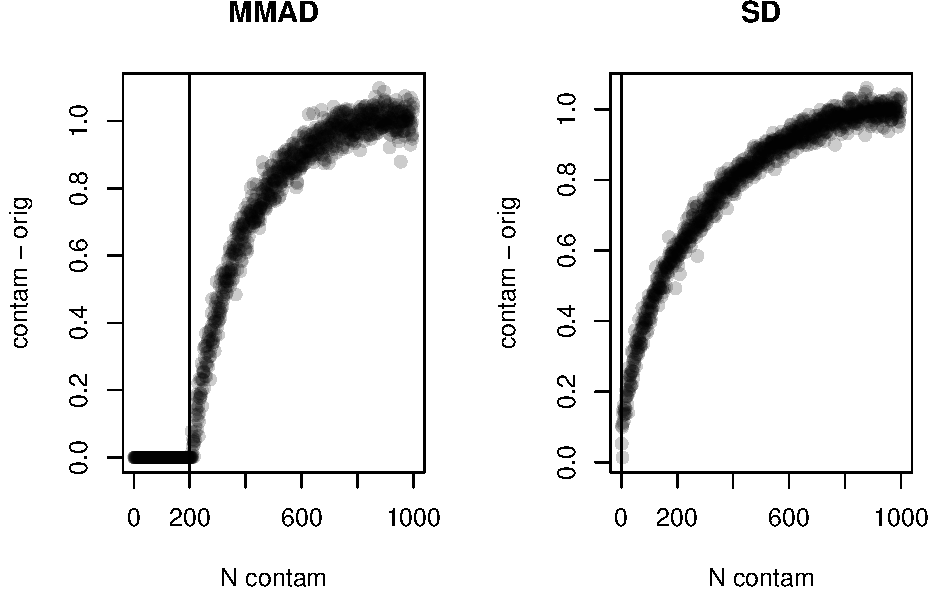
\includegraphics{effect_supplement_files/figure-latex/R-block-4-1.pdf}
\caption{The breakdown point is the percent contamination that can be
introduced into a distribution without changing the measure of scale.
The breakdown point of the MMAD is about 0.2, while the breakdown point
of the standard deviation is 0. The vertical lines indicate the
breakdown points.}
\end{figure}

\hypertarget{comparing-mathcalz-and-cohens-d}{%
\subsection{\texorpdfstring{Comparing \(\mathcal{Z}\) and Cohen's
d}{Comparing \textbackslash{}mathcal\{Z\} and Cohen's d}}\label{comparing-mathcalz-and-cohens-d}}

Finally, we examine how \(\mathcal{Z}\) and Cohen's d compare when
determining the standardized difference between two distributions. The
code is shown in \texttt{R-block-5} and Figure 4 shows how the two
statistics compare for Normal and Cauchy distributions, with an expected
difference of 2 and a scale parameter of 1.

Figure 4 shows that as expected Cohen's d had a standardized effect size
that was distributed around the mean value of 2.0 when two Normal
distributions were compared. The \(\mathcal{Z}\) standardized effect
size was distributed around a mean value of 1.4, which is expected given
that the denominator of \(\mathcal{Z}\) is 1.418 times larger than the
pooled standard deviation of 1. Applying this correction, the
standardized effect size for \(\mathcal{Z}\) would be 2.0, the same as
Cohen's d for a Normal distribution. Thus as instantiated, the
\(\mathcal{Z}\) is more conservative than Cohen's d, but can be easily
scaled if needed. Scaling is not performed by default, since there is no
guarantee that we are comparing Normal distributions in high throughput
sequencing datasets.

\begin{figure}
\centering
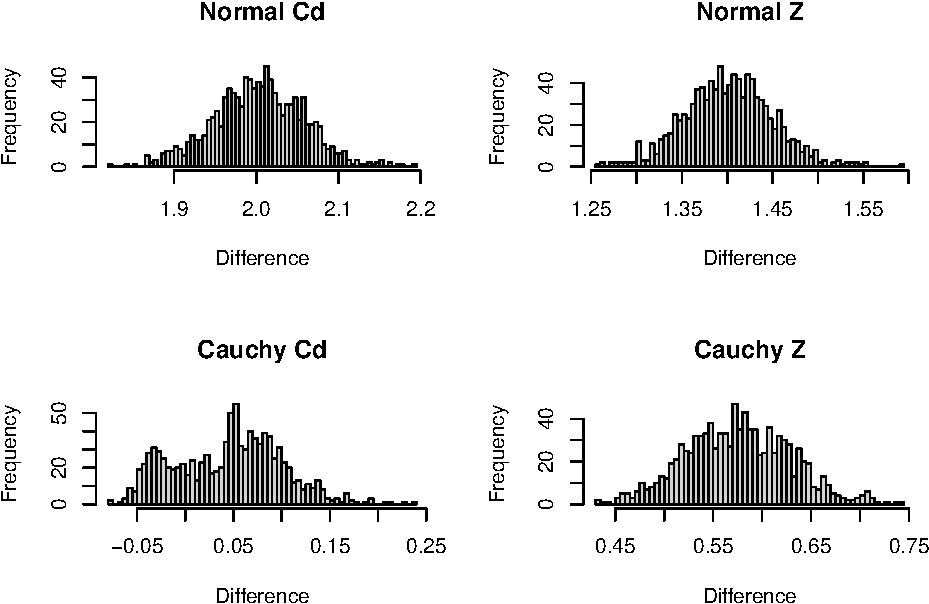
\includegraphics{effect_supplement_files/figure-latex/R-block-5-1.pdf}
\caption{The standardized effect size of \(\mathcal{Z}\) and Cohen's d
(Cd) are compared for Normal and Cauchy distributions. The histograms
plot one thousand random tests of the effect size for distributions of
size 1000. The difference between the distributions was set at 2 with a
scale parameter of 1 in each case.}
\end{figure}

The situation is very different when using the standardized effect size
to compare two Cauchy distributions. Here the mean effect size for
Cohen's d is 0.044, or almost no effect. Figure 4 shows that this
distribution is bimodal, and the median standardized effect is 0.046.
However, the \(\mathcal{Z}\) metric gives a mean standardized effect
size of 0.58 and is symmetrically distributed over a comparatively
narrow range. Recall that Cauchy distributions have very broad tails,
and so a scale of 1 with a Cauchy distribution will result in a
considerably broader distribution than will a Normal distribution with
the same scale, and consequently the standardized effect size should be
smaller than observed with a Normal distribution with the same location
and scale parameters.

\clearpage

We can also examine the relationship between the effect size and the
overlap between distributions, or more correctly the proportion of
distribution 1 that is greater than the midpoint of distribution 2. This
is reported in ALDEx2 as the `overlap'. In the case of Cohen's d, this
follows a nice relationship that is derived from the Normal
distribution, and the ideal relationship is plotted in the figure below
as the red dotted line.

In the case of ALDEx2, we show the values for the individual points from
the selex demonstration dataset. For the most part, the individual
points fall nicely along the anticipated line, but become a little
ragged at around \(\mathcal{Zeta}\) 1.5-2 as we approach the tails of
the distribution. We can also calculate the 95\% confidence interval for
\(\mathcal{Zeta}\), and the features where the CI does not cross 0 are
identified by the blue dots. We can see that some features have large
\(\mathcal{Zeta}\) scores, but not consistent scores. This is because
these features include outliers that give the dispersion distribution a
fat tail.

This shows that the measure of effect size used here has similar
distributional properties as does Cohen's d, and further cements the
utility and interpretability of the metric.

\begin{figure}
\centering
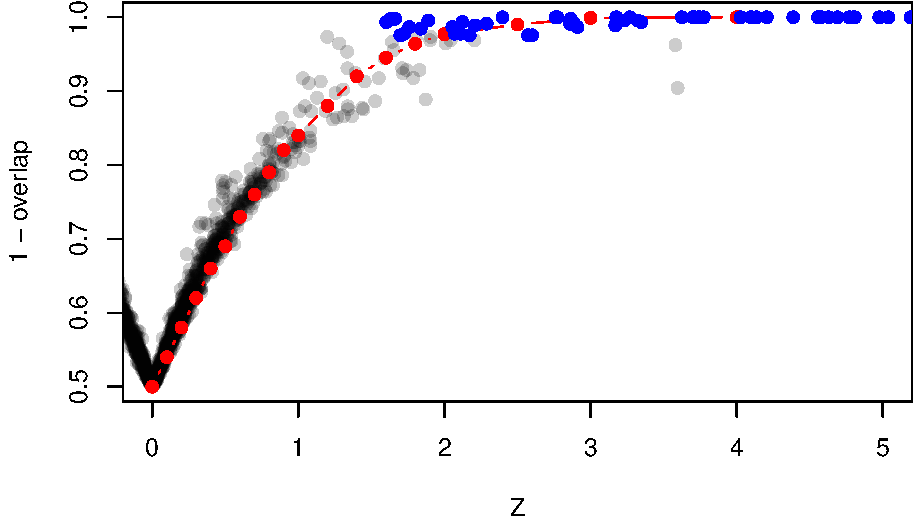
\includegraphics{effect_supplement_files/figure-latex/R-overlap-1.pdf}
\caption{Plot of \(\mathcal{Z}\) vs the distributional overlap. The red
points indicate the ideal values for Cohen's d in a Normal distribution,
the grey are points for the selex test dataset, and the blue points are
points from this dataset where the 95\% CI does not cross 0.}
\end{figure}

\clearpage

\hypertarget{the-null-model}{%
\subsection{The NULL model}\label{the-null-model}}

Figure 5 and associated code in \texttt{R-Block-dist} show the
underlying distributions used in Figure 1 in the main paper. This figure
shows the shape of the distributions used to determine the NULL model
graphs. We show here a single random instance of the 40 x 40 comparison
where the estimated \(\mathcal{Z}\) value is 1 in a Normal distribution.

\begin{figure}
\centering
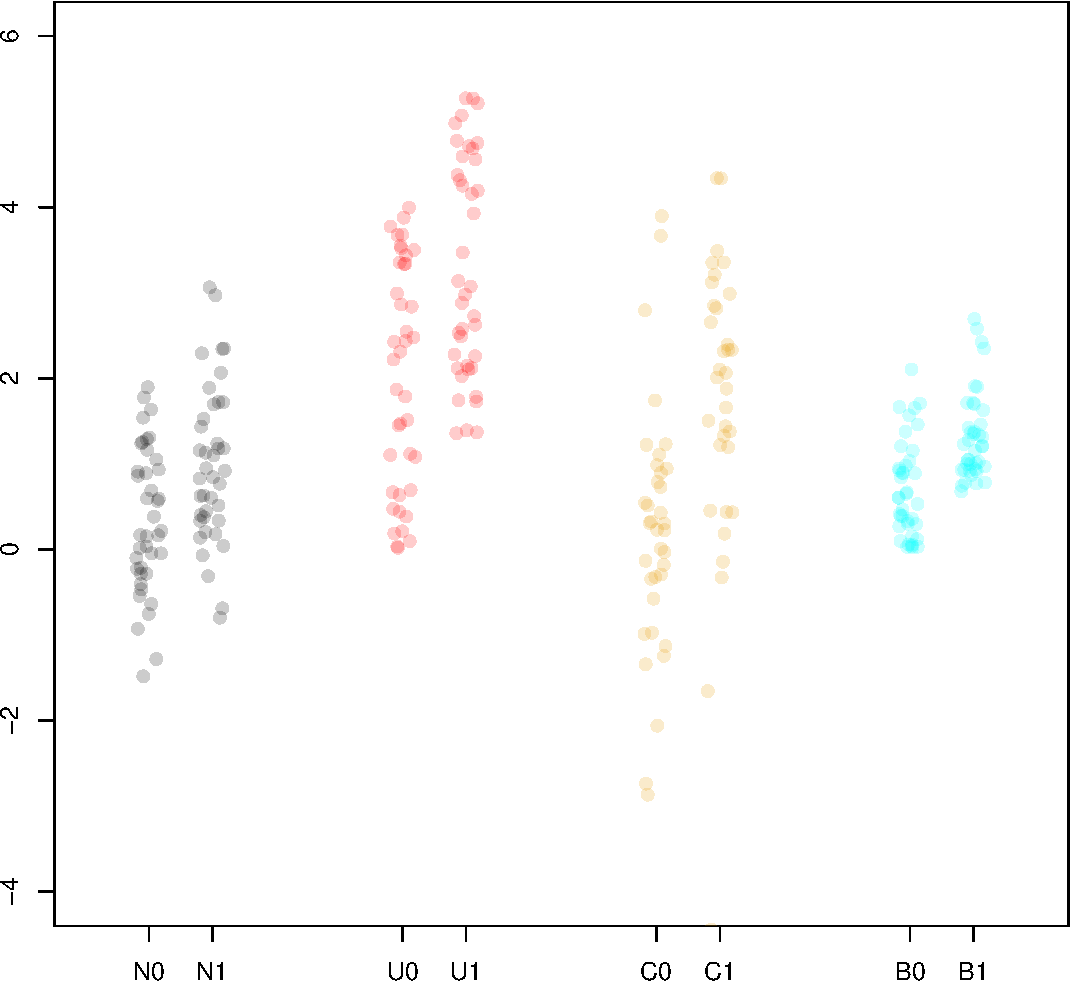
\includegraphics{effect_supplement_files/figure-latex/R-Block-dist-1.pdf}
\caption{Example distributions. Random samples of size 40 were drawn
from Normal (N), Uniform (U), Cauchy (C) or Beta (B) distributions.
Distributions were either the base distribution (0), or perturbed by a
small amount (1). Distribtions pairs are color coded using the same
colors as in Figure 1 in the main manuscript.}
\end{figure}

\clearpage

\hypertarget{the-yeast-transcriptome-dataset}{%
\section{The yeast transcriptome
dataset}\label{the-yeast-transcriptome-dataset}}

The main manuscript shows the results for a well-described transcriptome
dataset from a SNF1 \emph{Saccharomyces cerevisae} gene knockout with a
cutoff of \(\mathcal{Z} > 1 \mathrm{\ or\ } 2\). Later we expand on this
analysis and show a similar analyses from a 16S rRNA gene sequencing
experiment in a Chinese population.

\hypertarget{p-value-based-approaches}{%
\subsection{p-value based approaches}\label{p-value-based-approaches}}

We used the \emph{Saccharomyces cerevisia} 48-replicate SNF2 gene
knockout dataset described in (Schurch \emph{et al.}, 2016). We first
used the \texttt{CoDaSeq\ R} package to remove outlier samples using a
robust compositionally appropriate process (Peter \emph{et al.}, 2009),
which selects those samples that are further from all other samples than
expected. The actual approach is to generate the compositionally
appropriate Aitchison distance matrix after centered log-ratio
transformation (Aitchison, 1986) and to identity the total distance
between all samples in each group. Those samples that contribute more
than twice the interquartile range to the total distance of the matrix
are removed. Using this approach we removed samples 6, \emph{10}, 13,
\emph{15}, 25, \emph{31}, and 35 from the SNF2 group, leaving 41
``clean'' samples, and we removed samples 21,25,28,34 and 36 from the WT
group leaving 43 samples (samples that are removed by this approach but
were not removed in the (Schurch \emph{et al.}, 2016) dataset are in
italics). Sample 22 was not removed by this approach from the SNF2
group, but was using the approach in (Gierliński \emph{et al.}, 2015).
In general, this approach is slightly more aggressive in removing
outliers that was used in outliers than the one used in (Gierliński
\emph{et al.}, 2015; Schurch \emph{et al.}, 2016). Discrepencies between
the methods will largely occur because of the
compositionally-appropriate method adopted here (Aitchison, 1986). In
the dataset used here there were 6236 genes rather than the larger
number in the original report; the number of features is not expected to
alter the conclusions. The code is for this step is in
\texttt{code/setup.r}.

\begin{verbatim}
## Warning in kable_pipe(x = structure(c("Tool", "edgeR", "edgeR", "edgeR", : The
## table should have a header (column names)
\end{verbatim}

\begin{longtable}[]{@{}llll@{}}
\caption{TP set by method.}\tabularnewline
\toprule
\endhead
Tool & Method & Total genes & Significant genes\tabularnewline
edgeR & glm & 6349 & 4705\tabularnewline
edgeR & et & 6349 & 4684\tabularnewline
edgeR & et \& T\textgreater{}2 & 6349 & 101\tabularnewline
ALDEx2 & Wilcox & 6236 & 4318\tabularnewline
ALDEx2 & Welch's & 6236 & 4352\tabularnewline
ALDEx2 & \(\mathcal{Z}\) \textgreater{} 1 & 6236 & 2020\tabularnewline
ALDEx2 & \(\mathcal{Z}\) \textgreater{} 2 & 6236 & 545\tabularnewline
\bottomrule
\end{longtable}

Following the original report, we used the set of genes identified by
each tool with the full set of samples as the gold standard set. Table 1
shows the number of significant genes by each method. We can see that
the edgeR methods and the ALDEx2 p-value based methods return similar
sets of genes at an FDR cutoff of \(q < 0.05\). In fact, the different
toolsets return almost the same set of genes, with 4060 of the genes
being found by the four the p-value based approaches. The two
\(\mathcal{Z}\) cutoffs return a subset of the p-value based core set.
Note that filtering by p-value and fold-change is extraordinarily
restrictive: only 101 genes pass the p-value filter and a Threshold of
\textgreater{} 2 as defined in Gierlinski et al (2015), and indeed, the
Threshold of \textgreater{} 2 is all that is needed to identify that set
of 101 genes in this dataset.

\clearpage

\begin{figure}
\centering
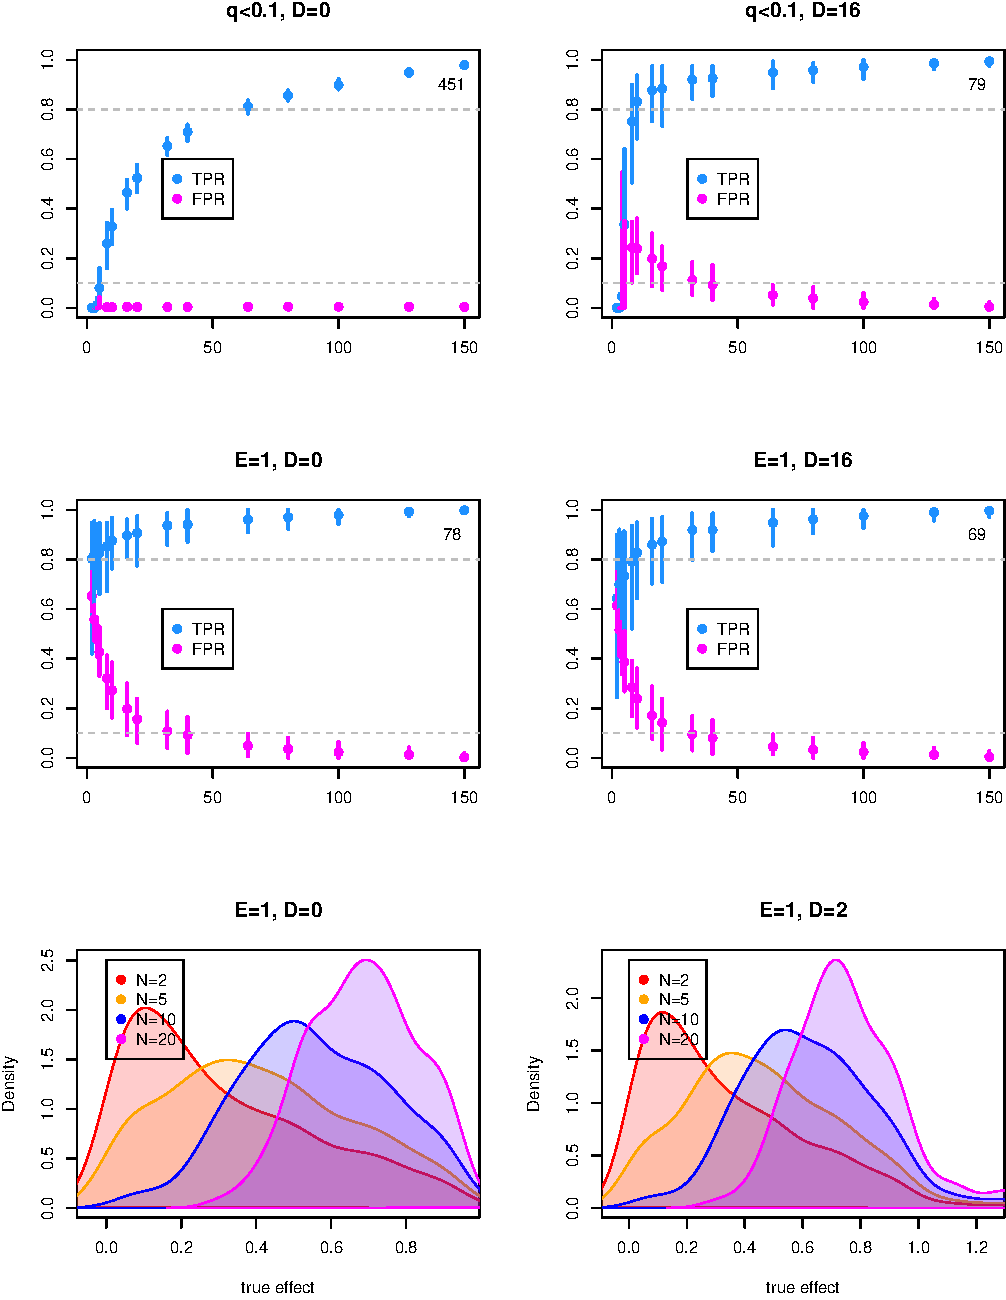
\includegraphics{effect_supplement_files/figure-latex/R-Block-ty-fptp-1.pdf}
\caption{Comparing Ed and adjusted p-values when detecting differential
features between two groups in a 16S rRNA gene sequencing dataset. The
top four panels show the median and 95\% confidence interval of the true
positive rate (TPR) and false positive rate (FPR) at different cutoff
values. The top two panels show the values for the q-value, the
Benjamini-Hochberg corrected p-value, as a function of sample size. The
middle two panels show the values for Ed. Data were summarized using
either a 0 or 16-fold difference cutoff (D). The number of features of
non-o features that are identified as significantly different in the
full dataset are shown in the top left corner of each plot. The bottom
two panels show the effect size distribution of features identified as
false positives by Ed at four different sample sizes. The dashed grey
lines show the cutoff for a 10\% FDR and an 80\% power to detect.}
\end{figure}

We reproduce the analyses in a 16S rRNA gene sequencing dataset (Bian
\emph{et al.}). Here we compared microbial composition of the 8-12 year
old cohort (161 samples) to the young soldier cohort (211 samples) using
the OTU count table published as supplement to the paper. As before, 100
ALDEx2 instances were conducted to identify the set of OTUs that are
found reproducibly. Data derived from 16S rRNA gene sequencing of
communities is similar in many ways to transcriptome data, but are
inherently noisier and generally sparser than transcriptome data
(Fernandes \emph{et al.}, 2014; Gloor \emph{et al.}, 2016, 2017). Thus,
these data provide an independent test of the generality of the
conclusions outlined above.

We first replicate Figure 2 of the main manuscript using
\(\mathcal{Z} > 1 \mathrm{, and} > 1\), and the results are shown in
Figure 6 and the code is in code block \texttt{R-Block-ty-fptp}. Large
effect sizes are uncommon in microbiome datasets (Falony \emph{et al.},
2016; Tsilimigras and Fodor, 2016) because the dispersion is extreme as
shown in Figure 7. The code for this is contained in
\texttt{R-block-ty-volcano}.

The left panel in Figure 7 shows the relationship between dispersion
(diff.win from ALDEx2) and relative abundance (rab.all from ALDEx2) for
the yeast transcriptome and the 16S rRNA gene sequencing dataset. Tthe
transcriptome dataset has a strong relationship, where the most abundant
transcripts tend to have extremely low dispersion, and the rarest
features (those near the low-count margin) have the greatest dispersion.
In contrast, the relationship between abundance and dispersion is nearly
uncoupled in the 16S rRNA gene sequencing dataset.

\begin{figure}
\centering
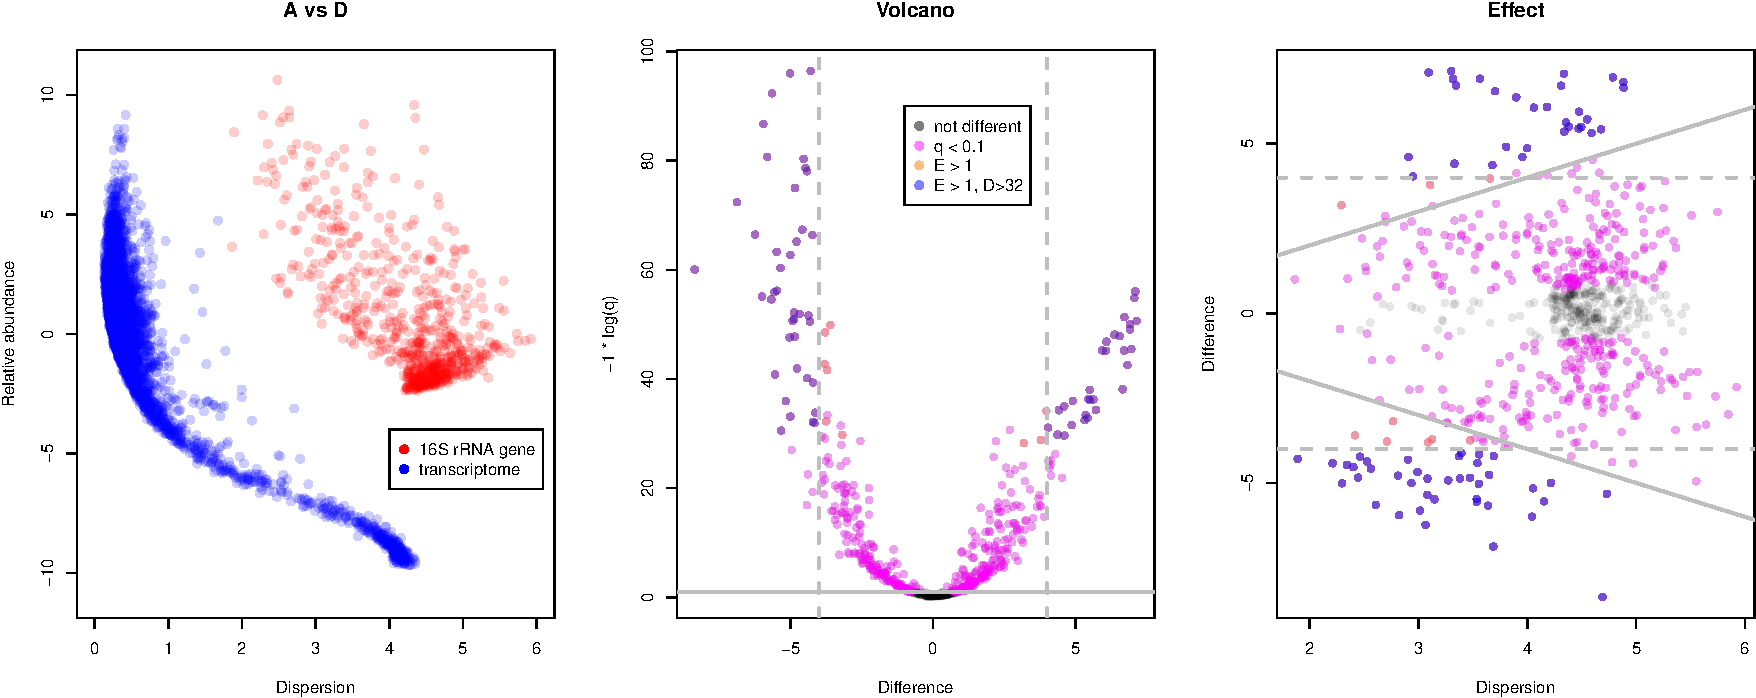
\includegraphics{effect_supplement_files/figure-latex/R-block-ty-volcano-1.pdf}
\caption{Abundance vs.~Dispersion, Volcano and Effect plots. The A vs D
plot shows the relationship between the dispersion in the dataset
vs.~the relative abundance for the yeast transcriptome dataset in the
main text, and the 16S rRNA gene sequencing dataset. Dispersion is the
MMAD for each feature, and the Relative abundance is the median of the
clr-transformed Dir Monte-Carlo instances (rab.all and diff.win from
ALDEx2). The Volcano and Effect plots show features identified by Ed ,
adjusted p-values and absolute differences when detecting differential
features between two groups for the 16S rRNA gene sequencing dataset.
These plots compare the features identified by Ed and by q-scores and a
16-fold fold-change thresholds in the full dataset. This large absolute
fold change is required as the within-group dispersion is enormous in
this and other 16S rRNA gene sequencing datasets. In these plots all
features that have a q score less than 0.1 also have an effect size
greater than 1. Thus, the features in magenta are only identified as
significantly different by q scores, those in orange are significantly
different by both their q score and their effect size, and features in
blue are significant by their q score, their effect size and their
absolute difference. The dashed grey lines in the two plots demarcate
the 16-fold difference location; note that the difference is in a log2
scale. The horizontal solid line in the Volcano plot indicates a FDR (q
score) of 0.1. The diagonal solid lines in the Effect plot indicate the
boundary where the difference equals the dispersion; ie, where the
effect size is 1.}
\end{figure}

\clearpage

Finally, \texttt{R-block-how-many} and Figure 8 shows the TP-FP
characteristics of the two real datasets and the simulated datasets. For
this we superimposed the 99th percentile of effect sizes from subsets of
the 16S rRNA gene sequencing dataset or form the transcriptome dataset
where comparison groups were randomly sampled from the same group. Thus,
this analysis accounts for biological and sampling variation, and the
simulated datasets include only sampling variation. The \(\mathcal{Z}\)
values for the randomly sub-sampled data were computed in two ways.
First, using the clr-transformed point estimates of the data, and second
using the clr-transformed Bayesian posterior distributions of the data.
No difference between group was expected. We see that the point estimate
values from the real data overlap almost exactly with the point estimate
values from the simulated data, indicating that the simulated data is a
good proxy for the actual biological data. Interestingly, the 99th
percentile of \(\mathcal{Z}\) derived from the expected value of the
Bayesian posterior estimate is significantly more conservative than the
point-estimate derived statistic. In this case, \(\mathcal{Z}\) values
of 2 or more are likely reasonable regardless of the sample size or
dataset, and using a cutoff of \(\mathcal{Z}\) of 1 is likely to be a
safe threshold as long as the sample size per group is at least 10.

\begin{figure}
\centering
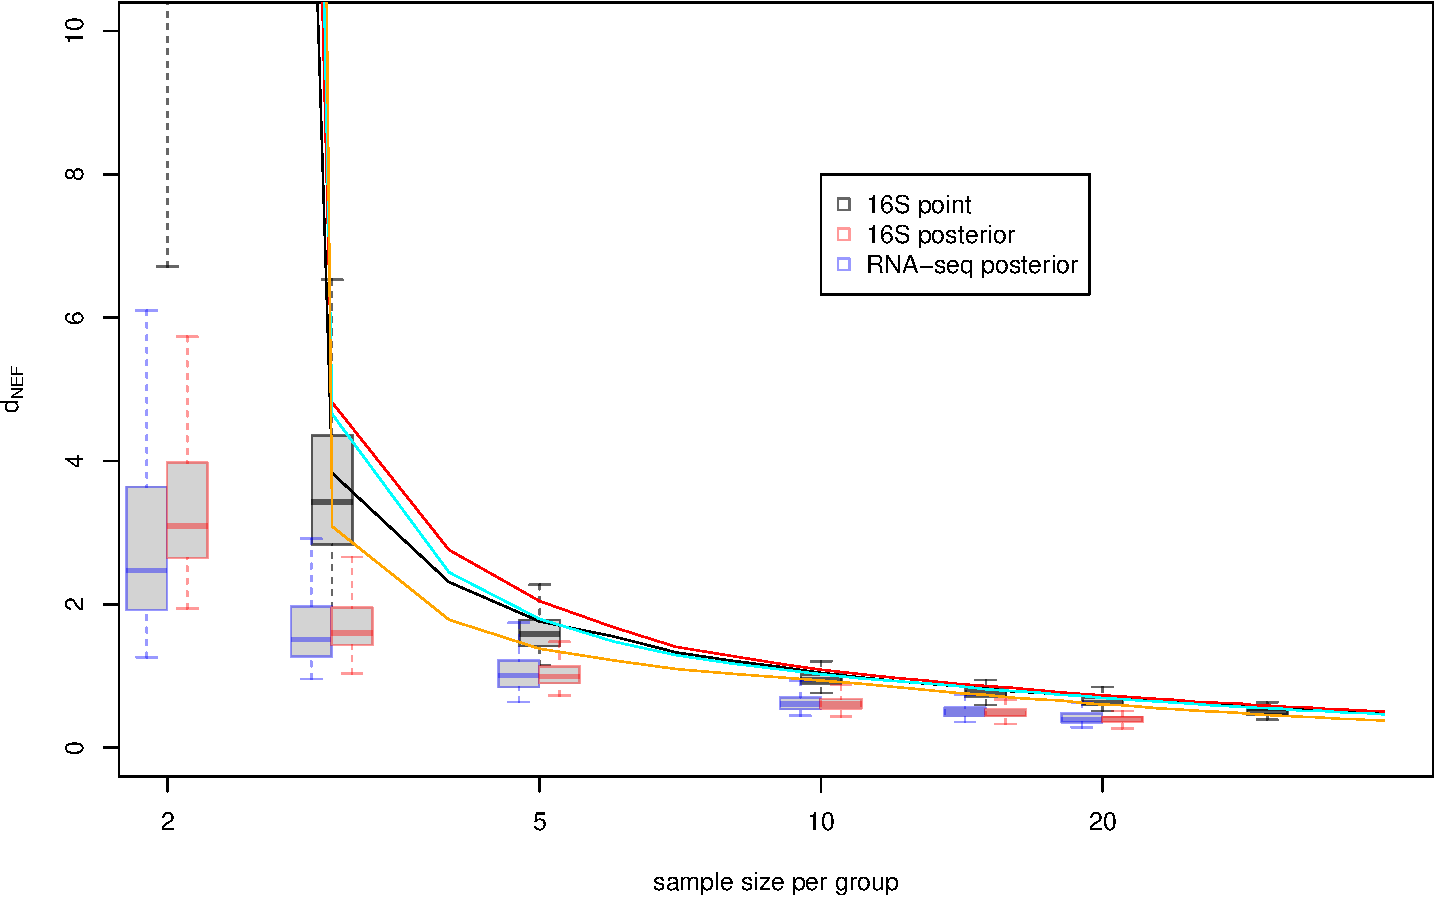
\includegraphics{effect_supplement_files/figure-latex/R-block-how-many-1.pdf}
\caption{The proportion of features that have an effect size
\(\mathcal{Z}\) as a function of per-group sample size when there is
known to be no true effect. The line graphs show plots of the same data
as in Figure 1; these are the 99th percentile effect sizes from Normal,
Cauchy, Uniform and Beta random distributions. The boxplots overlay the
99th percentile effect sizes from subsets of the 16S rRNA gene
sequencing dataset or the transcriptome dataset where groups were
randomly sampled from the same group, and thus no difference between
group was expected. Sample sizes were chosen up to a maximum of one half
the total number of samples per group. The plots show boxplots of the
99th percentile of the effect size of 100 subsets per sample size.}
\end{figure}

\clearpage

\hypertarget{references}{%
\section*{References}\label{references}}
\addcontentsline{toc}{section}{References}

\hypertarget{refs}{}
\leavevmode\hypertarget{ref-Aitchison:1986}{}%
Aitchison,J. (1986) The statistical analysis of compositional data
Chapman \& Hall, London, England.

\leavevmode\hypertarget{ref-Anders:2013aa}{}%
Anders,S. \emph{et al.} (2013) Count-based differential expression
analysis of RNA sequencing data using R and Bioconductor. \emph{Nat
Protoc}, \textbf{8}, 1765--86.

\leavevmode\hypertarget{ref-Anders:2015aa}{}%
Anders,S. \emph{et al.} (2015) HTSeq--a python framework to work with
high-throughput sequencing data. \emph{Bioinformatics}, \textbf{31},
166--9.

\leavevmode\hypertarget{ref-bian:2017}{}%
Bian,G. \emph{et al.} The gut microbiota of healthy aged chinese is
similar to that of the healthy young. \emph{mSphere}, \textbf{2},
e00327--17.

\leavevmode\hypertarget{ref-cohen_effect}{}%
Cohen,J. (2013) Statistical power analysis for the behavioral sciences
Academic press.

\leavevmode\hypertarget{ref-Cui:2003aa}{}%
Cui,X. and Churchill,G.A. (2003) Statistical tests for differential
expression in cDNA microarray experiments. \emph{Genome Biol},
\textbf{4}, 210.1--210.10.

\leavevmode\hypertarget{ref-Falony:2016aa}{}%
Falony,G. \emph{et al.} (2016) Population-level analysis of gut
microbiome variation. \emph{Science}, \textbf{352}, 560--4.

\leavevmode\hypertarget{ref-fernandes:2013}{}%
Fernandes,A.D. \emph{et al.} (2013) ANOVA-like differential expression
(aldex) analysis for mixed population rna-seq. \emph{PLoS One},
\textbf{8}, e67019.

\leavevmode\hypertarget{ref-fernandes:2014}{}%
Fernandes,A.D. \emph{et al.} (2014) Unifying the analysis of
high-throughput sequencing datasets: Characterizing RNA-seq, 16S rRNA
gene sequencing and selective growth experiments by compositional data
analysis. \emph{Microbiome}, \textbf{2}, 15.1--15.13.

\leavevmode\hypertarget{ref-Gierlinski:2015aa}{}%
Gierliński,M. \emph{et al.} (2015) Statistical models for rna-seq data
derived from a two-condition 48-replicate experiment.
\emph{Bioinformatics}, \textbf{31}, 3625--3630.

\leavevmode\hypertarget{ref-gloorFrontiers:2017}{}%
Gloor,G.B. \emph{et al.} (2017) Microbiome datasets are compositional:
And this is not optional. \emph{Front Microbiol}, \textbf{8}, 2224.

\leavevmode\hypertarget{ref-gloorAJS:2016}{}%
Gloor,G.B. \emph{et al.} (2016) Compositional uncertainty should not be
ignored in high-throughput sequencing data analysis. \emph{Austrian
Journal of Statistics}, \textbf{45}, 73--87.

\leavevmode\hypertarget{ref-Hedges:1985}{}%
Hedges,L.V. and Olkin,I. (1985) Statistical methods for meta-analysis
Academic Press, Orlando.

\leavevmode\hypertarget{ref-Jiang:2011aa}{}%
Jiang,L. \emph{et al.} (2011) Synthetic spike-in standards for rna-seq
experiments. \emph{Genome Res}, \textbf{21}, 1543--51.

\leavevmode\hypertarget{ref-bowtie2}{}%
Langmead,B. and Salzberg,S.L. (2012) Fast gapped-read alignment with
bowtie 2. \emph{Nature methods}, \textbf{9}, 357--359.

\leavevmode\hypertarget{ref-macklaim:2013}{}%
Macklaim,J.M. \emph{et al.} (2013) Comparative meta-RNA-seq of the
vaginal microbiota and differential expression by lactobacillus iners in
health and dysbiosis. \emph{Microbiome}, \textbf{1}, 12.

\leavevmode\hypertarget{ref-filmozer:2009}{}%
Peter,F. \emph{et al.} (2009) Principal component analysis for
compositional data with outliers. \emph{Environmetrics}, \textbf{20},
621--632.

\leavevmode\hypertarget{ref-Schurch:2016aa}{}%
Schurch,N.J. \emph{et al.} (2016) How many biological replicates are
needed in an rna-seq experiment and which differential expression tool
should you use? \emph{RNA}, \textbf{22}, 839--51.

\leavevmode\hypertarget{ref-Tsilimigras:2016aa}{}%
Tsilimigras,M.C.B. and Fodor,A.A. (2016) Compositional data analysis of
the microbiome: Fundamentals, tools, and challenges. \emph{Ann
Epidemiol}, \textbf{26}, 330--5.

\end{document}
